\documentclass[aspectratio=169]{beamer}

%\includeonlyframes{current}

\usepackage[utf8]{inputenc}
\usepackage[american]{babel}
\usepackage{amsmath,amsthm}
\usepackage{booktabs}
\usepackage{ifthen}
\usepackage{tikz}
\usetikzlibrary{calc,arrows,arrows.meta,intersections,positioning,decorations.markings}
\usepackage{ulem}

\mode<presentation>{%
  \usetheme{ibm}
}

\title{A Personal History of Isogeny-based Cryptography}
\author{Luca De Feo}
\date[September 16, 2025, Nancy]{September 16, 2025\\
  Colloquium du Loria, Nancy
}
\institute{IBM Research Zürich}

\begin{document}

\frame[plain]{\titlepage}

%%

\begin{frame}{A brief history of elliptic curves in cryptography}
  \large
  \begin{description}
  \item<1->[1976] Diffie--Hellman key exchange
  \item<1->[1977] RSA
  \item<2->[1985] Miller and Koblitz introduce elliptic curves to cryptography
  \item<4->[1994] Shor's quantum algorithm
  \item<6->[1997] Couveignes' isogeny-based key exchange
  \item<3->[1999] NIST standardizes its first elliptic curves
  \item<5->[2017] NIST calls for post-quantum algorithms
  \end{description}
\end{frame}

%%

\begin{frame}
  \LARGE
  \begin{center}
    \only<1>{\emph{Cryptographie et isogenies: une histoire française}}
    \only<2>{\includegraphics[height=\textheight]{defunes}}
    \only<3>{\includegraphics[height=\textheight]{slip-francais}}
  \end{center}
\end{frame}

%%

\begin{frame}{Diffie--Hellman key exchange (1976)}
  \large
  
  \begin{center}
    \emph{Setup:} A cyclic group $G=\langle g\rangle$.
  \end{center}

  \bigskip
  
  \begin{center}
    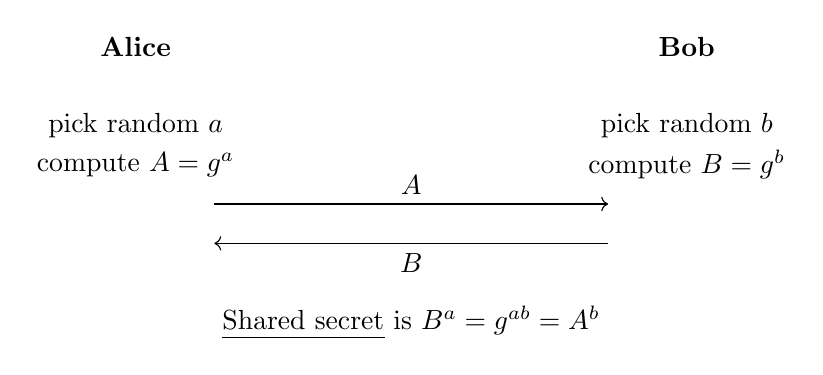
\begin{tikzpicture}
      \node at (0,0) {\bf Alice};
      \node at (7,0) {\bf Bob};
      \node at (0,-1) {pick random \alert{$a$}};
      \node at (0,-1.5) {compute $A=g^a$};
      \node at (7,-1) {pick random \alert{$b$}};
      \node at (7,-1.5) {compute $B=g^b$};
      \draw[->]
      (1,-2) to node[auto] {$A$} (6,-2);
      \draw[->] (6,-2.5) to node[auto] {$B$} (1,-2.5);
      \node at (3.5,-3.5) {\emph{Shared secret} is \alert{$B^a=g^{ab}=A^b$}};
    \end{tikzpicture}
  \end{center}
\end{frame}

%%

\begin{frame}{Elliptic curves}
  \begin{columns}
    \begin{column}{0.4\textwidth}
      \Large\centering
      $y^2 = x^3 + ax + b$
    \end{column}
    \begin{column}{0.6\textwidth}
      \begin{center}
        \begin{tikzpicture}[domain=-2.4566:4,samples=100,yscale=1/2]
          \draw plot (\x,{sqrt(\x*\x*\x-4*\x+5)});
          \draw plot (\x,{-sqrt(\x*\x*\x-4*\x+5)});

          \begin{uncoverenv}<2->
            \draw (-3,1) -- (4,8/3+3);
            \begin{scope}[every node/.style={draw,circle,inner sep=1pt,fill},cm={1,2/3,0,0,(0,3)}]
              \node at (-2.287980,0) {};
              \node at (-0.535051,0) {};
              \node at (3.267475,0) {};
            \end{scope}
            \begin{scope}[every node/.style={yshift=0.3cm},cm={1,2/3,0,0,(0,3)}]
              \node at (-2.287980,0) {$P$};
              \node at (-0.535051,0) {$Q$};
              \node at (3.267475,0) {$R$};
            \end{scope}

            \draw[dashed] (3.267475,3.267475*2/3+3) -- (3.267475,-3.267475*2/3-3) 
            node[draw,circle,inner sep=1pt,fill] {}
            node[xshift=-0.1cm,anchor=east] {$P\oplus Q$};
          \end{uncoverenv}
        \end{tikzpicture}
      \end{center}
    \end{column}
  \end{columns}
\end{frame}

%%

\begin{frame}{What's needed for key exchange?}
  \begin{columns}
    \begin{column}{0.5\textwidth}
      \centering
      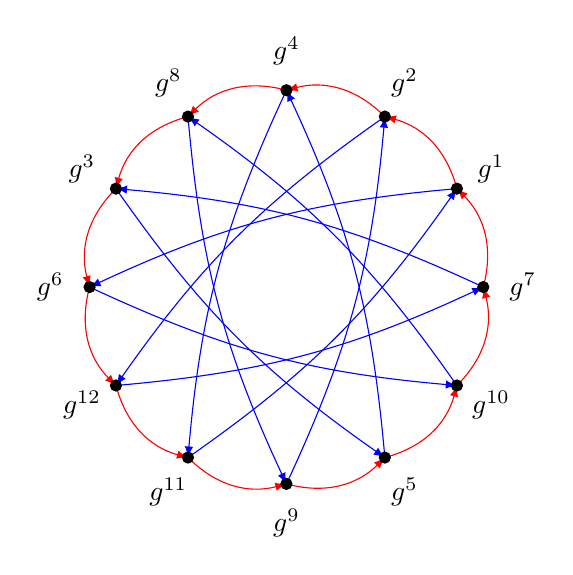
\begin{tikzpicture}
        \def\crater{12}
        \def\jumpa{5}
        \def\diam{2.5cm}

        \foreach \i in {1,...,\crater} {
          \draw[red,-latex] (360/\crater*\i : \diam) to[bend right] (360/\crater*\i+360/\crater : \diam);
          \draw[blue,-latex] (360/\crater*\i : \diam) to[bend right=10] (360/\crater*\i+\jumpa*360/\crater : \diam);
        }

        \foreach \i in {1,...,\crater} {
          \pgfmathparse{int(mod(pow(2,\i-1),\crater+1))}
          \let\e\pgfmathresult
          \draw[fill] (360/\crater*\i: \diam) circle (2pt) +(360/\crater*\i: 0.5) node{$g^{\e}$};
        }
      \end{tikzpicture}
    \end{column}
    \begin{column}{0.4\textwidth}

      \begin{itemize}
      \item[\sout{prod:}] \sout{$g^ag^b = g^{a+b}$,}
      \item[exp:] $(g^a)^b = g^{ab} = (g^b)^a$.
      \end{itemize}

      \bigskip
      The hard problem:
      \begin{itemize}
      \item[dlog:] $g^a \mapsto a$.
      \end{itemize}
    \end{column}
  \end{columns}
\end{frame}

%%

\begin{frame}
  \centering\Large
  \begin{description}
    \setlength{\itemsep}{4em}
  \item[Isogenies =] finite-kernel \textit{algebraic} group morphisms of elliptic curves
  \item[Endomorphisms =] isogenies \emph{$E \to E$}
  \end{description}
\end{frame}

%%

\begin{frame}
  \Large\centering
  \begin{tikzpicture}[remember picture,overlay,shift=(current page.center)]
    \node (E) at (-4,1) {\alt<1>{$E$}{$\bullet$}};
    \node (E1) at (4,1) {\alt<1>{$E'$}{$\bullet$}};
    \draw[-latex] (E) edge node[above] {\only<1>{$\phi$}} (E1);
    \uncover<3->{\node at (0,-1) {Isogenous};}
  \end{tikzpicture}
\end{frame}

%%

\begin{frame}
  \centering
  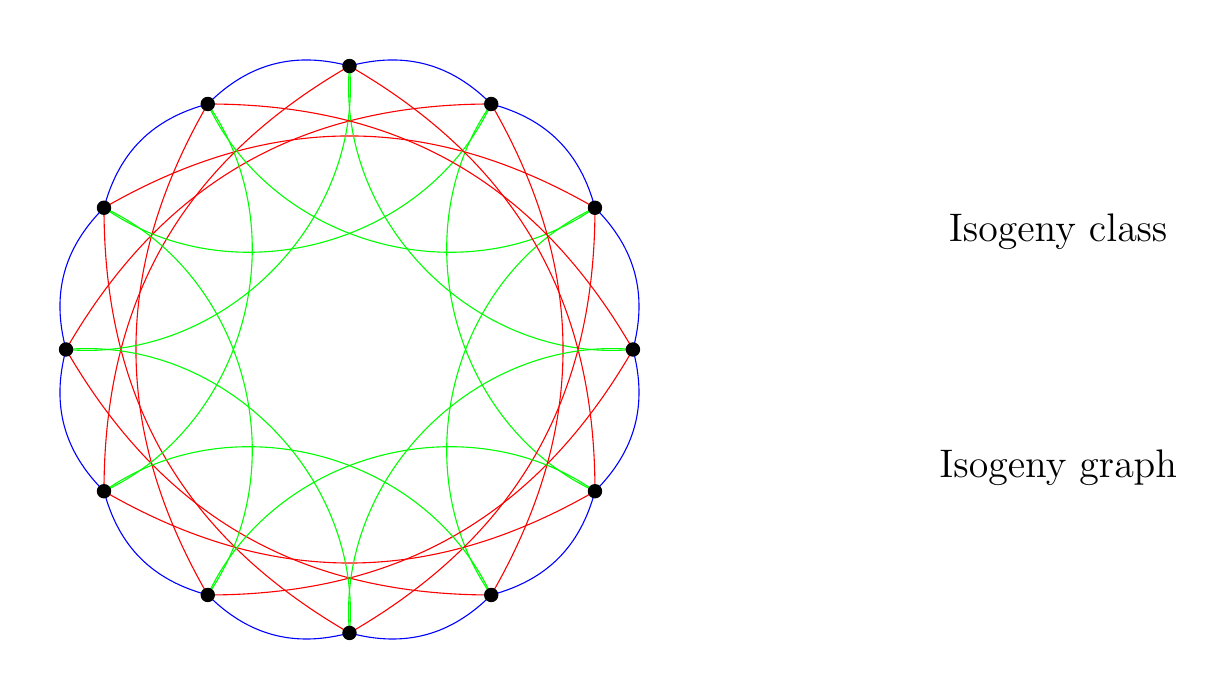
\begin{tikzpicture}
    \begin{scope}[scale=1.2]
      \def\crater{12}
      \def\jumpa{-8}
      \def\jumpb{9}
      \def\diam{3cm}

      \uncover<2->{
        \foreach \i in {1,...,\crater} {
          \draw[blue] (360/\crater*\i : \diam) to[bend right] (360/\crater*\i+360/\crater : \diam);
          \draw[red] (360/\crater*\i : \diam) to[bend right] (360/\crater*\i+\jumpa*360/\crater : \diam);
          \draw[green] (360/\crater*\i : \diam) to[bend right=50] (360/\crater*\i+\jumpb*360/\crater : \diam);
        }
      }
      \foreach \i in {1,...,\crater} {
        \draw[fill] (360/\crater*\i: \diam) circle (2pt) +(360/\crater*\i: 0.4);
      }
    \end{scope}

    \begin{scope}
      \Large
      \uncover<1->{\node at (9,1.5) {Isogeny class};}
      \uncover<2->{\node at (9,-1.5) {Isogeny graph};}
    \end{scope}
  \end{tikzpicture}
\end{frame}

%%

\begin{frame}{The isogeny problem}
  \Large\centering
  \begin{tikzpicture}
    \node (E) at (0,0) {$E$};
    \node (E1) at (8,0) {$E'$};
    \uncover<2->{
      \draw[-latex] (E) edge node[above] {??} (E1);
    }
  \end{tikzpicture}
\end{frame}

%% 

\begin{frame}{Isogenies as ``exponents''}
  \begin{columns}
    \begin{column}{0.55\textwidth}
      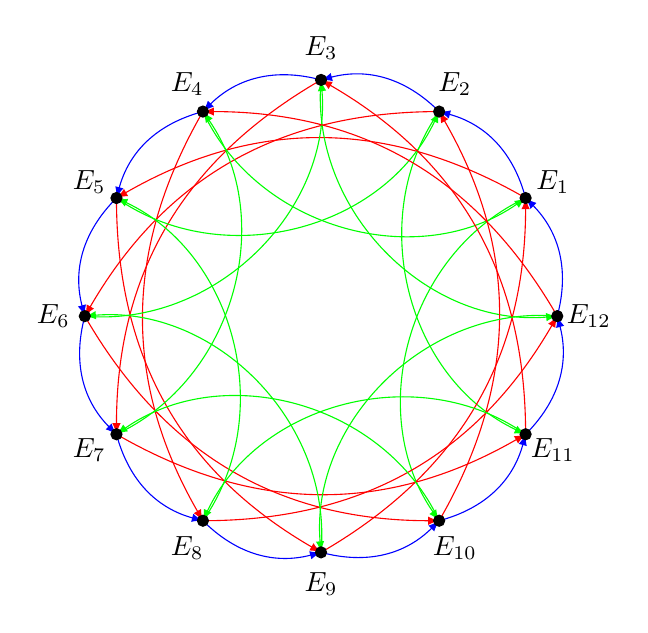
\begin{tikzpicture}
        \begin{scope}
          \def\crater{12}
          \def\jumpa{-8}
          \def\jumpb{9}
          \def\diam{3cm}

          \foreach \i in {1,...,\crater} {
            \draw[blue,-latex] (360/\crater*\i : \diam) to[bend right] (360/\crater*\i+360/\crater : \diam);
            \draw[red,-latex] (360/\crater*\i : \diam) to[bend right] (360/\crater*\i+\jumpa*360/\crater : \diam);
            \draw[green,-latex] (360/\crater*\i : \diam) to[bend right=50] (360/\crater*\i+\jumpb*360/\crater : \diam);
          }
          \foreach \i in {1,...,\crater} {
            \draw[fill] (360/\crater*\i: \diam) circle (2pt) +(360/\crater*\i: 0.4) node{$E_{\i}$};
          }
        \end{scope}
      \end{tikzpicture}
    \end{column}
    \begin{column}{0.45\textwidth}
      \large
      \begin{description}
        \setlength{\itemsep}{1em}
      \item<3->[Commutative]
        $E^{(\textcolor{red}{\bullet}\textcolor{blue}{\bullet})} = E^{(\textcolor{blue}{\bullet}\textcolor{red}{\bullet})}$
      \item<2->[Group]
        $(E^{\textcolor{red}{\bullet}})^{\textcolor{blue}{\bullet}} = E^{(\textcolor{red}{\bullet}\textcolor{blue}{\bullet})}$
      \item[Action]
        $E_2 = E_1^{\textcolor{blue}{\bullet}}$\\
        $E_5 = E_1^{\textcolor{red}{\bullet}}$\\
        $E_{10} = E_1^{\textcolor{green}{\bullet}}$
      \end{description}
    \end{column}
  \end{columns}
\end{frame}

%%

\begin{frame}{Couveignes' key exchange (1997)}
  \begin{center}
    \emph{Setup:} A group of isogenies, a starting curve $E_0$ defined over $\mathbb{F}_p$
  \end{center}

  \bigskip
  
  \begin{center}
    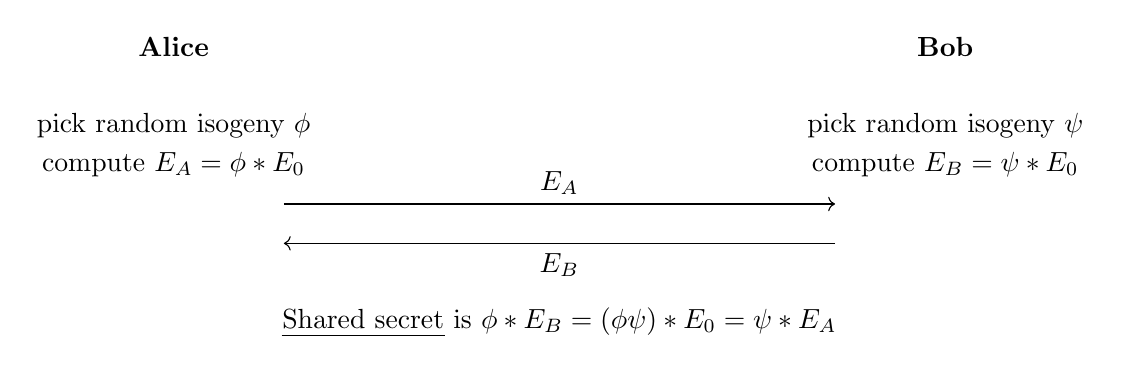
\begin{tikzpicture}[x=1.4cm]
      \node at (0,0) {\bf Alice};
      \node at (7,0) {\bf Bob};
      \node at (0,-1) {pick random isogeny \alert{$\phi$}};
      \node at (0,-1.5) {compute $E_A=\phi*E_0$};
      \node at (7,-1) {pick random isogeny \alert{$\psi$}};
      \node at (7,-1.5) {compute $E_B=\psi*E_0$};
      \draw[->]
      (1,-2) to node[auto] {$E_A$} (6,-2);
      \draw[->] (6,-2.5) to node[auto] {$E_B$} (1,-2.5);
      \node at (3.5,-3.5) {\emph{Shared secret} is \alert{$\phi*E_B=(\phi\psi)*E_0=\psi*E_A$}};
    \end{tikzpicture}
  \end{center}
\end{frame}

%%

\begin{frame}
  \centering
  \begin{tabular}{c c}
    \includegraphics[width=0.25\textwidth]{fm}
    & \includegraphics[width=0.7\textwidth]{isogeny-party-2006}
  \end{tabular}
\end{frame}

%%

\begin{frame}
  \begin{tikzpicture}
    \node at (0,0) {\includegraphics[width=\textwidth]{ecc2009-prog}};
    \uncover<2->{\draw[red,very thick,-latex] (4,-3) -- (2.5,-3.5);}
    \uncover<3->{\draw[red,very thick,-latex] (4,-0.5) -- (2.5,-1);}
  \end{tikzpicture}
\end{frame}

%%

\begin{frame}
  \begin{columns}
    \begin{column}{0.3\textwidth}
      \small \emph{Source:}
      D. J. Bernstein,\\
      \textit{``Post-quantum cryptography''},\\
      2009, Calgary, Canada
    \end{column}
    \begin{column}{0.7\textwidth}
      \includegraphics[height=\textheight]{ecc2009-bernstein}
    \end{column}
  \end{columns}
\end{frame}

%%

\begin{frame}[plain]
  \includegraphics[width=\textwidth]{rockies}
\end{frame}

%%

\begin{frame}{David Jao's summer of 2010}
  \begin{columns}
    \begin{column}{0.4\textwidth}
      \centering
      \includegraphics[height=0.9\textheight]{djao}
    \end{column}
    \begin{column}{0.6\textwidth}
      \large
      With A. Childs and V. Soukharev:
      \begin{itemize}
      \item Inverting group action $\Leftrightarrow$ Hidden shift problem
      \item Solved in \emph{quantum subexponential time} by Kuperberg's algorithm
      \item[$\Rightarrow$] Couveigne's key exchange is dead
      \end{itemize}

      \bigskip
      
      Hires me as a postdoc:
      \begin{quotation}
        ``I had this idea for a key exchange to replace
        Couveignes'. What do you think of it?''
      \end{quotation}
    \end{column}
  \end{columns}
\end{frame}

%%

\begin{frame}{Degree of an isogeny}
  \begin{columns}
    \large
    \begin{column}{0.5\textwidth}
      \centering
      \[\deg(\phi) \in \mathbb{N}^+\]

      \begin{itemize}
      \item A measure of ``size'';
      \item<2-> \emph{Multiplicative;}
      \item<3-> A measure of ``complexity'':\\
        only isogenies of small degree fit into a computer!
      \end{itemize}
    \end{column}
    \begin{column}{0.5\textwidth}
      \centering
      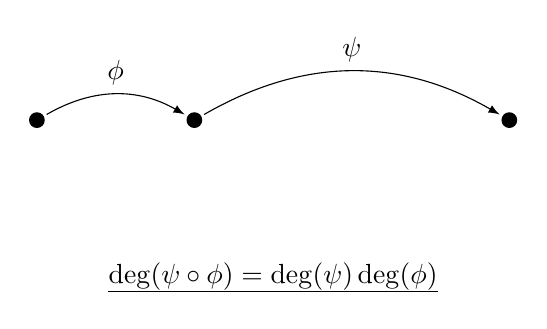
\begin{tikzpicture}
        \fill
        (0,0) circle (1mm) node(A){}
        ++(2,0) circle (1mm) node(B){}
        ++(4,0) circle (1mm) node(C){};
        \draw[-latex]
        (A) edge[bend left] node[above]{$\phi$} (B)
        (B) edge[bend left] node[above]{$\psi$} (C);

        \uncover<2->{
          \node at (3,-2) {\emph{$\deg(\psi\circ\phi) = \deg(\psi)\deg(\phi)$}};
        }
      \end{tikzpicture}
    \end{column}
  \end{columns}
\end{frame}

%%

\begin{frame}{The 2-isogeny graph}
  \Large
  \begin{columns}
    \begin{column}{0.45\textwidth}
      \centering
      degree
      \only<1>{$2$}%
      \only<2>{$4$}%
      \only<3>{$8$}%
      \only<4>{$16$}%
      \only<5>{$2^x$}
    \end{column}
    \begin{column}{0.55\textwidth}
      \centering
      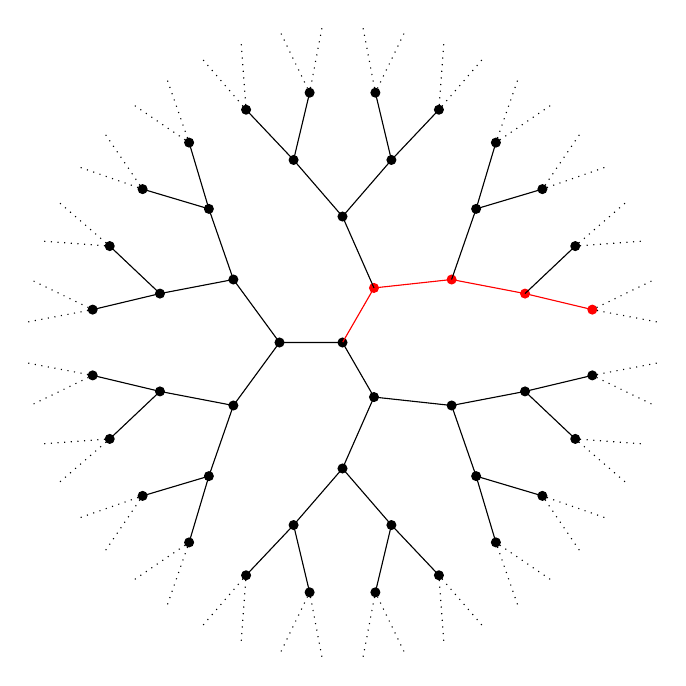
\begin{tikzpicture}[scale=0.8]
        \def\levels{5}
        \draw[fill] (0:0) circle (2pt);
        \foreach \i in {1,...,\levels} {
          \pgfmathparse{3*2^\i}
          \let\nodes\pgfmathresult
          \foreach \j in {1,3,...,\nodes} {
            \pgfmathparse{\j + (-1)^div(\j,2)}
            \let\lower\pgfmathresult
            \uncover<\i->{
              \ifthenelse{\i = \levels}{
                \draw[dotted] (360/\nodes*\j : \i) --
                (360/\nodes*\lower : \i - 1);
              }{
                \pgfextra{
                  \ifthenelse{\j=1}{\def\col{red}}{\def\col{black}}
                  \draw[fill,\col] (360/\nodes*\j : \i) circle (2pt) --
                  (360/\nodes*\lower : \i - 1);
                }
              }
            }
          }
        }
      \end{tikzpicture}
    \end{column}
  \end{columns}
\end{frame}

%%

\begin{frame}{Elliptic curves over a finite field}
  \large\centering
  \begin{tabular}{l@{~~~~}c@{~~~~}c}
    & \emph{Ordinary} & \emph{Supersingular}\\
    \hline
    & common & rare\\
    \emph{Cardinality} & unpredictable & predictable\\
    \emph{Isogeny classes} & many & one\\
    \emph{Group action} & yes & no\\
    \emph{$\ell$-Isogeny graph} & cycles & $(\ell+1)$-regular, connected\\
    \emph{Expander graph} & many $\ell$ together & single $\ell$\\
  \end{tabular}
\end{frame}

%%

\begin{frame}
  \includegraphics[width=\textwidth]{PathFinding}
\end{frame}

%%

\begin{frame}{Supersingular Isogeny Diffie--Hellman (SIDH)}
  \Large\centering
  \begin{tikzpicture}
    \node (E) at (0,0) {$E$};
    \node (E1) at (8,0) {$E'$};
    \draw[-latex,red] (E) edge node[above] {??} (E1);
    \uncover<2->{
      \node at (0,-1) {$P_1, P_2, \ldots, P_n$};
      \node at (8,-1) {$\phi(P_1), \phi(P_2), \ldots, \phi(P_n)$};
      \node at (4,-3) {\emph{$n \gg \deg\phi$}};
    }
  \end{tikzpicture}
\end{frame}

%%

\begin{frame}[plain]
  \centering
  \includegraphics[width=\textwidth]{ecc2011-group}
\end{frame}

%%

\begin{frame}
  \centering
  \includegraphics[width=\textwidth]{ecc2011-schedule}  
\end{frame}

%%

\begin{frame}
  \begin{columns}
    \begin{column}{0.6\textwidth}
      \centering
      \uncover<1->{\includegraphics[height=0.55\textheight]{sidh-pre-ecc}}

      \bigskip
      
      \uncover<3->{\includegraphics[height=0.3\textheight]{sidh-post-ecc}}
    \end{column}
    \begin{column}{0.4\textwidth}
      \centering
      \uncover<2->{\includegraphics[height=0.95\textheight]{ecc2011-me}}
    \end{column}
  \end{columns}
\end{frame}

%%

\begin{frame}
  \centering

  \begin{tikzpicture}[node distance=0,anchor=north east]
    \node{\includegraphics[width=0.3\textwidth]{ecc2011-tomato.jpg}};
    \node{\includegraphics[width=0.8\textwidth]{ecc2011-xtomato-scrot.png}};
  \end{tikzpicture}
    
  \bigskip
  $\to$ \alert{\url{https://web.archive.org/web/20201122222657/http://ecc2011.loria.fr/tomato.html}} $\leftarrow$
\end{frame}

%%

{
  \setbeamercolor{background canvas}{bg=black}
  \setbeamercolor{frametitle}{fg=white!70!black}
  \begin{frame}[plain]
    \begin{tikzpicture}[remember picture,overlay,white]
      \large\bf
      \node(pic)[at=(current page.center)] {
        \includegraphics[width=\paperwidth]{ecc2011-xtomato.jpg}
      };
    \end{tikzpicture}
  \end{frame}
}

%%

\begin{frame}{NIST Post-quantum Standardization (2017)}
  \begin{quotation}\
    [\dots]
    
    Due to this concern, many researchers have begun to investigate
    post-quantum cryptography (PQC) (also called quantum-resistant or
    quantum-safe cryptography). \emph{The goal of this research is to
    develop cryptographic algorithms that would be secure against both
    quantum and classical computers}. These algorithms could serve as
    replacements for our current public-key cryptosystems to prepare
    for the eventuality that large-scale quantum computers become a
    reality.

    [\dots]
    
    At present, there are several post-quantum cryptosystems that have
    been proposed, \emph{including lattice-based cryptosystems,
      code-based cryptosystems, multivariate cryptosystems, hash-based
      signatures, and others}. However, for most of these proposals,
    further research is needed in order to gain more confidence in
    their security (particularly against adversaries with quantum
    computers) and to improve their performance.

    [\dots]
  \end{quotation}
\end{frame}

%%

\begin{frame}[plain]
  \includegraphics[width=\textwidth]{sike-page}
\end{frame}

%%

\begin{frame}[plain]
  \centering
  \includegraphics[width=\textwidth]{ecc2017-program}
\end{frame}

%%

\begin{frame}{Resurrecting Couveignes' key exchange}
  \begin{columns}
    \begin{column}{0.4\textwidth}
      \centering
      \includegraphics[height=0.8\textheight]{jean-kieffer}
    \end{column}
    \begin{column}{0.6\textwidth}
      \medskip
      \begin{description}
      \item[Why:] A quantum subexponential attack is \textbf{not a total
          break}.
      \item[Why:] Security of group action key exchange is based on
        \textbf{purer problems}.
      \item[Jean's MSc thesis:] All the tricks from the SIDH
        book + new ideas\\
        \uncover<2->{$\to$ \emph{5 minutes for a key exchange\dots}}
      \end{description}
    \end{column}
  \end{columns}
\end{frame}

%%

\begin{frame}[plain]
  \centering
  \includegraphics[width=\textwidth]{csidh-ec2018-rump}
\end{frame}

%%

\begin{frame}{The CSIDH subgraph}
  \begin{columns}
    \begin{column}{0.4\textwidth}
      \centering\large
      \begin{itemize}
        \setlength{\itemsep}{1em}
      \item Easy to reach and recognize
      \item Same properties as an ordinary graph\\
        $\to$ Group action!
      \item<2-> \emph{40ms for a key exchange!}
      \end{itemize}
    \end{column}
    \begin{column}{0.6\textwidth}
      \centering
      \includegraphics[height=0.9\textheight]{gfp-subgraph}
    \end{column}
  \end{columns}
\end{frame}

%%

\begin{frame}{In the meantime: cryptanalysis on SIDH / SIKE}
  \begin{columns}
    \begin{column}{0.7\textwidth}
      \begin{description}
      \item[2014] Kohel--Lauter--Petit--Tignol (KLPT):\\
        ``Quaternionic versions'' of isogeny problems are easy
      \item[2016] Galbraith--Petit--Shani--Ti:\\
        Man-in-the-middle attack on SIDH
      \item[2017] Petit:\\
        ``Overstreched'' variants of SIDH are easy
      \item[2018] Eisentraeger--Hallgren--Lauter--Morrison--Petit
      \item[2021] Wesolowski:\\
        supersingular isogeny problem $\Leftrightarrow$ endomorphism ring problem
      \end{description}
    \end{column}
    \begin{column}{0.3\textwidth}
      \centering
      \uncover<2->{
        \includegraphics[width=0.9\textwidth]{christophe-petit}
        \small Christophe Petit
      }
    \end{column}
  \end{columns}
\end{frame}

%%

\begin{frame}{The Deuring correspondence(s)}
  \centering\large
  \setlength{\tabcolsep}{2em}
  \renewcommand{\arraystretch}{1.8}
  \begin{tabular}{r l}
    \emph{Ellitpic curves} & \emph{Number fields / Quaternion algebras}\\
    \hline
    Endomorphisms & Algebraic integers\\
    Endomorphism ring & (Maximal) order\\
    Isogeny & Ideal\\
    Isogeny degree & Ideal norm\\
    Isogeny composition & Ideal multiplication\\
    \color{gray}Isogenies \raisebox{-0.8em}{\tikz{\node (E) at (0,0) {$\bullet$}; \node (E1) at (2,0) {$\bullet$}; \draw[->] (E) edge[bend left] (E1) edge[bend right] (E1);}} & \color{gray}Ideal classes\\
    \color{gray}Dual isogeny & \color{gray}Conjugate ideal\\
  \end{tabular}
\end{frame}

%%

\begin{frame}[plain]
  \centering
  \includegraphics[height=\textheight]{cycle-leman}
\end{frame}

%%

\begin{frame}{It's 2018 and still no decent isogeny-based signature\dots}
  \uncover<2->{
    \begin{tabular}{c c}
      \includegraphics[height=0.8\textheight]{benjamin-wesolowski}
      &  \Large Not for long!
    \end{tabular}
  }
\end{frame}

%%

\begin{frame}[plain]
  \centering
  \includegraphics[height=\textheight]{post-scryptum}
\end{frame}

%%

\begin{frame}{SQIsign (De Feo, Kohel, Leroux, Petit, Wesolowski 2020)}
  \begin{columns}
    \begin{column}{0.3\textwidth}
      \begin{itemize}
      \item First \emph{compact} post-quantum signature (< RSA)
      \item Based on supersingular isogenies
      \item Constructive use of Deuring correspondence
      \end{itemize}
    \end{column}
    \begin{column}{0.7\textwidth}
      \textbf{SQIsign v1 (NIST submission, June 2023)}
      \begin{table}[h]
        \centering
        \begin{tabular}{c r r r r r}
          \toprule
          & \multicolumn{2}{c}{Sizes (bytes)} & \multicolumn{3}{c}{Timings (ms)}\\
          \cmidrule(lr){2-3}\cmidrule(lr){4-6}
          Security & Public Key & Signature & Keygen & Sign & Verify \\
          \midrule
          NIST-1 &  64 & 177 &  1,864 &  2,890 &    54 \\
          NIST-3 &  96 & 263 & 11,867 & 21,880 &   327 \\
          NIST-5 & 128 & 335 & 45,525 & 79,272 & 1,089 \\
          \midrule
        \end{tabular}
      \end{table}
    \end{column}
  \end{columns}
\end{frame}

%%

\begin{frame}{NIST's first batch of finalists (June 2022)}
  \Large
  
  To be standardized:
  \begin{itemize}
  \item 3 lattice-based
  \item 1 hash-based
  \end{itemize}

  Kept for possible future standardization:
  \begin{itemize}
  \item 3 code-based
  \item SIKE
  \end{itemize}
\end{frame}

%%

\begin{frame}[plain]
  \centering
  \begin{tikzpicture}[remember picture,overlay]
    \node[at=(current page.center)] {
      \includegraphics[width=\paperwidth]{nist-celebrate.jpg}
    };
  \end{tikzpicture}
\end{frame}

%% 

\begin{frame}[plain]
  \includegraphics[width=\textwidth]{craigs-mail.png}
\end{frame}

%%

\begin{frame}[plain]
  \centering
  \begin{tikzpicture}[remember picture,overlay]
    \node[at=(current page.center)] {
      \includegraphics[width=\paperwidth]{quantamag.png}
    };
  \end{tikzpicture}
\end{frame}

%%

\begin{frame}[plain]
  \centering
  \begin{tikzpicture}[remember picture,overlay]
    \node[at=(current page.center)] {
      \includegraphics[width=\paperwidth]{nist-edit.jpg}
    };
  \end{tikzpicture}
\end{frame}

%%

\begin{frame}{Higher dimensional abelian varieties}
  \centering
  \begin{tikzpicture}[domain=-2.4566:4,samples=100]
    \begin{scope}[xscale=0.3,yscale=0.5]
      \draw plot (\x,{sqrt(\x*\x*\x-4*\x+5)});
      \draw plot (\x,{-sqrt(\x*\x*\x-4*\x+5)});
      \node (P1) at (3,4.47213595499958) {};
    \end{scope}
    \begin{uncoverenv}<2->
      \begin{scope}[xscale=0.7,yscale=0.15,shift={(7,-20)}]
        \draw plot ({sqrt(\x*\x*\x-4*\x+5)},\x);
        \draw plot ({-sqrt(\x*\x*\x-4*\x+5)},\x);
        \node (P2) at (-4.47213595499958,3) {};
      \end{scope}
      \node at (5,0) {\huge $E \times E$};
      
      \fill (P1) circle (2pt);
      \fill (P2) circle (2pt);

      \draw[dashed] (P2) -- (P2 |-, |- P1) -- (P1);
      \fill (P2 |-, |- P1) circle (2pt) node[above right] {$(P,Q)$};
    \end{uncoverenv}
  \end{tikzpicture}
\end{frame}

%%

\begin{frame}{Higher dimensional isogenies}
  \large
  \begin{columns}
    \begin{column}{0.4\textwidth}
      \centering
      \begin{tikzpicture}[scale=2]
        \uncover<2->{
          \node (A) at (-1,1) {$A$};
          \node (B) at (1,-1) {$B$};
          \node (C) at (1,1) {$C$};
          \node (D) at (-1,-1) {$D$};
          
          \draw[-latex] (A) edge node[above] {$\alpha$} (C) edge node[left] {$\beta$} (D)
          (B) edge node[right] {$\gamma$} (C) edge node[below] {$\delta$} (D);
        }
      \end{tikzpicture}
    \end{column}
    \begin{column}{0.6\textwidth}
      \begin{align*}
        \Phi : A \times B &\to C \times D\\
        \uncover<2->{(P,Q) &\mapsto \bigl( \alpha(P) + \gamma(Q), \beta(P) + \delta(Q) \bigr)}\\
              &\uncover<3->{=
                \begin{pmatrix}
                  \alpha&\gamma\\\beta&\delta
                \end{pmatrix}
                \begin{pmatrix}
                  P\\Q
                \end{pmatrix}}
      \end{align*}

      \medskip

      \begin{uncoverenv}<4->
        \Large
        \[
          \emph{\deg\Phi =
            \det\left(\begin{smallmatrix}
              \alpha&\gamma\\\beta&\delta
            \end{smallmatrix}\right)}
        \]
      \end{uncoverenv}
    \end{column}
  \end{columns}
\end{frame}

%%

\begin{frame}{Isogeny-based crypto goes HD}
  \large
  \begin{description}
    \setlength{\itemsep}{1em}
  \item[2023] SQIsignHD (Dartois--Leroux--Robert--Wesolowski)
  \item[2023] FESTA (Basso--Maino--Pope)
  \item[2023] QFESTA (Nakagawa--Onuki)
  \item[2023] SCALLOP-HD (Chen--Leroux--Panny)
  \item[2024] SQIsign2D-West (Basso--De
    Feo--Dartois--Leroux--Maino--Pope--Robert--Wesolowski)
  \item[2024] SQIsign2D-East (Nakagawa--Onuki)
  \item[2024] SQIPrime (Duparc--Fouotsa)
  \item \dots
  \end{description}
\end{frame}

%%

\begin{frame}{SQIsign is still running!}

  \centering

  \textbf{SQIsign v1 (June 2023)}
  \begin{table}[h]
    \centering
    \begin{tabular}{c r r r r r}
      \toprule
      & \multicolumn{2}{c}{Sizes (bytes)} & \multicolumn{3}{c}{Timings (ms)}\\
      \cmidrule(lr){2-3}\cmidrule(lr){4-6}
        Security & Public Key & Signature & Keygen & Sign & Verify \\
      \midrule
        NIST-1 &  64 & 177 &  1,864 &  2,890 &    54 \\
        NIST-3 &  96 & 263 & 11,867 & 21,880 &   327 \\
        NIST-5 & 128 & 335 & 45,525 & 79,272 & 1,089 \\
      \midrule
    \end{tabular}
  \end{table}

  \vspace{.5em}
  \textbf{SQIsign v2 (June 2025)}
  \begin{table}[h]
    \centering
    \begin{tabular}{c r r r r r}
      % \toprule
      % & \multicolumn{2}{c}{\phantom{Sizes (bytes)}} & \multicolumn{3}{c}{\phantom{Timings (ms)}}\\[-2em]
      % \cmidrule(lr){2-3}\cmidrule(lr){4-6}
      \phantom{Security} & \phantom{Public Key} & \phantom{Signature} & \phantom{Keygen} & \phantom{Sign} & \phantom{Verify} \\[-2em]
      \midrule
        NIST-1 &  66 & 148 &  25 &   60 &  3 \\
        NIST-3 &  98 & 222 &  67 &  161 &  9 \\
        NIST-5 & 130 & 294 & 119 &  300 & 18 \\
      \bottomrule
    \end{tabular}
  \end{table}  
\end{frame}

%%

\begin{frame}[plain]
  \centering
  \includegraphics[height=\textheight]{nancy-cycle}
\end{frame}

%%

\begin{frame}[plain]
  \centering
  \begin{tikzpicture}[remember picture,overlay]
    \begin{scope}[xscale=1.7,yshift=-15,opacity=0.8]
      \def\crater{12}
      \def\jumpa{-8}
      \def\jumpb{9}
      \def\diam{5cm}

      \foreach \i in {1,...,\crater} {
        \draw[blue] (360/\crater*\i : \diam) to[bend right] (360/\crater*\i+360/\crater : \diam);
        \draw[red] (360/\crater*\i : \diam) to[bend right] (360/\crater*\i+\jumpa*360/\crater : \diam);
        \draw[green] (360/\crater*\i : \diam) to[bend right=50] (360/\crater*\i+\jumpb*360/\crater : \diam);
      }
    \end{scope}
    
    \draw (0,0.5) node{\Huge\bf Thank you};
    \draw (0,-0.6) node{\large\url{https://defeo.lu/}};
    \draw (0,-1.3) node{\large\includegraphics[height=0.9em]{mastodon.png}~\href{https://twitter.com/luca_defeo}{@luca\_defeo@ioc.exchange}};
    \draw (0,-1.9) node{\large\includegraphics[height=0.9em]{bluesky.png}~\href{https://bsky.app/profile/bsky.defeo.lu}{@bsky.defeo.lu}};
  \end{tikzpicture}
\end{frame}

\end{document}


% LocalWords:  Isogeny abelian isogenies hyperelliptic supersingular Frobenius
% LocalWords:  isogenous
